% LuaLaTeX
\pdfvariable minorversion=7
\documentclass[10pt]{article}

% Packages
\usepackage[no-math]{fontspec}
\usepackage{geometry}
\usepackage{hyperref}
\usepackage[backend=biber]{biblatex} % we use the biber implementation of biblatex for bibliographies
%\usepackage[nonumberlist, toc]{glossaries}
\usepackage{graphicx}
\usepackage{pdfpages}
\usepackage{booktabs}
\usepackage{float}
\usepackage{subcaption}
\usepackage{fancyhdr}
\usepackage{amsmath}
\usepackage{siunitx}
\usepackage{multirow}

% Formatting
\geometry{letterpaper, portrait, margin=.85in}
\defaultfontfeatures{Ligatures=TeX}
\setmainfont[
    BoldFont       = Avenir Medium,
    ItalicFont     = Avenir Book Oblique,
    BoldItalicFont = Avenir Medium Oblique
]{Avenir Book}
\setmonofont{Andale Mono}
\sisetup{detect-all} % used by siunitx to always typeset units in the font of the current environment
\urlstyle{same}

\newcommand\theteamname{Midnight Sun Solar Car Team} % should not change normally
\newcommand\theuniversityname{University of Waterloo} % should also not change normally
\newcommand\theteamwebsite{www.uwmidsun.com} % should also not normally change
\newcommand\theteamphone{(519) 888-4567 x32978} % should also not normally change

\newcommand\thetitle{Battery Tech Report} % <--------------- add the title
\newcommand\thesubtitle{Electrical} % <--------------- add a subtitle or leave the field empty
\newcommand\theauthor{Minghao Ji} % <--------------- add an author with contact info or comment this line
\newcommand\theauthorcontact{minghao.ji@uwmidsun.com} % <--------------- add author's email or leave the field empty
\newcommand\thedate{\today} % <--------------- update the date, use this format

\pagestyle{fancy}
\renewcommand{\headrulewidth}{0pt}
\lhead{\thetitle}
\rhead{\theteamname}

\begin{document}

% Title Page
\begin{titlepage}
\large
\vspace*{2cm}
\centering

\includegraphics[width=.25\textwidth]{./figures/midnightSunLogoCircle.png} \\
\vspace{1.5cm}
{\LARGE \theteamname} \\
\theuniversityname \\
\vspace{2.2cm}
{\LARGE MSXII} \\
\vspace{0.4cm}
{\huge\bfseries \thetitle} \\
\vspace{0.2cm}
{\LARGE \thesubtitle} \\
\vspace{2.2cm}
\ifdefined \theauthor
\par Prepared by: \\
\theauthor \\
\theauthorcontact \\
\fi
\thedate \\
\vfill
\theteamwebsite \\
\theteamphone
\end{titlepage}

% Main Matter
\tableofcontents
%\listoffigures % <-------------- uncomment for list of figures
%\listoftables % <-------------- uncomment for list of tables

\newpage

\section{Battery Specifications}

\subsection{5.2.D.1: Manufacturer Information}

\begin{table}[!htbp]
\begin{tabular}{|l|l|}
\hline
\textbf{Manufacturer Name}      & LG Chemical Limited                                                                                                                   \\ \hline
\textbf{Manufacturer Contact}   & \begin{tabular}[c]{@{}l@{}}Jon Caserta, Liion Wholesale Batteries (Supplier)\\ support@liionwholesale.com\\ 888-972-2883\end{tabular} \\ \hline
\textbf{Cell Specification URL} & \url{http://vruzend.com/SpecificationINR18650MJ1.pdf}                                                                                 \\ \hline
\textbf{Cell MSDS URL}          & \url{http://www.batteryspace.com/prod-specs/6626_1.pdf}
\end{tabular}
\end{table}

\subsection{5.2.D.2: Stock Number}

\begin{table}[!htbp]
\begin{tabular}{|l|l|}
\hline
\textbf{Stock Number} & INR18650 MJ1 \\ \hline
\end{tabular}
\end{table}

\subsection{5.2.D.3: Cell \& Module Voltage}

\begin{table}[!htbp]
\begin{tabular}{|l|l|l|}
\hline
\textbf{Minimum (V)} & \textbf{Nominal (V)} & \textbf{Maximum (V)} \\ \hline
2.500                & 3.635                & 4.200                \\ \hline
\end{tabular}
\end{table}

\subsection{5.2.D.4: Bus Voltage}

\begin{table}[!htbp]
\begin{tabular}{|l|l|}
\hline
\textbf{Nominal (V)} & \textbf{Maximum (V)} \\ \hline
130.86               & 151.2                \\ \hline
\end{tabular}
\end{table}

\subsection{5.2.D.5: Pack Information}

\begin{table}[!htbp]
\begin{tabular}{|l|l|}
\hline
\textbf{Cells per module}    & 36   \\ \hline
\textbf{Modules per string}  & 36   \\ \hline
\textbf{Strings in parallel} & 1    \\ \hline
\textbf{Total cell count}    & 1296 \\ \hline
\end{tabular}
\end{table}

\subsection{5.2.D.6: Manufacturer's specifications}

\begin{table}[!htbp]
\begin{tabular}{|l|l|}
\hline
\textbf{Capacity (kWh)} & $\frac{3.5 \text{ Ah} \times 130.86 \text{ V} \times 36 \text{ modules}}{1000 \text{ Wh}} = 16.48836$ \\ \hline
\textbf{Weight (kg)}    & \begin{tabular}[c]{@{}l@{}}0.049 kg (max)\\ 0.049 kg \times 1296 = 63.50400 kg\end{tabular}           \\ \hline
\textbf{Cost (USD)}     & $\$ 3.88 \times 1296 = \$ 5028.48$                                                                    \\ \hline
\end{tabular}
\end{table}

\subsection{5.2.D.7: Spill/damage protocols and procedures}

See attached datasheet and MSDS

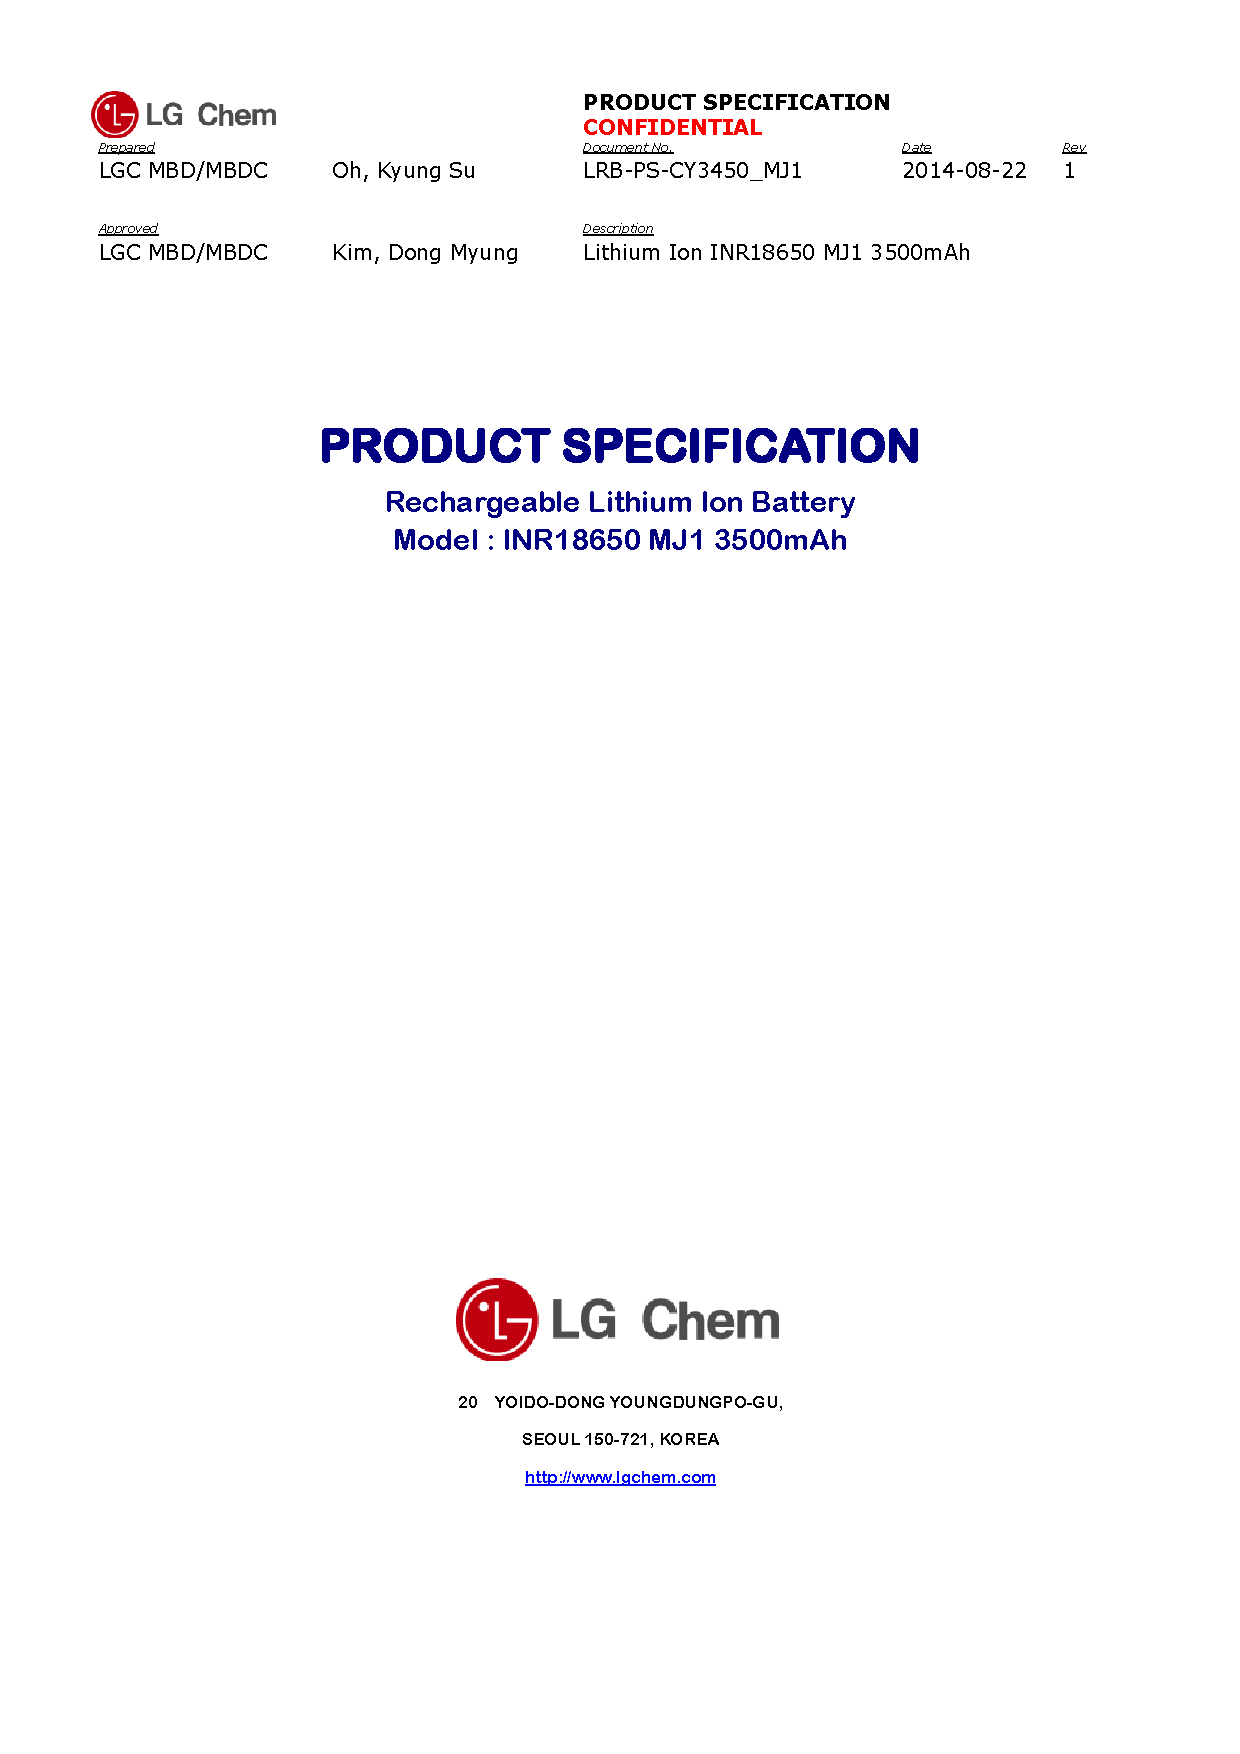
\includepdf[pages={-}]{forms/SpecificationINR18650MJ1.pdf}
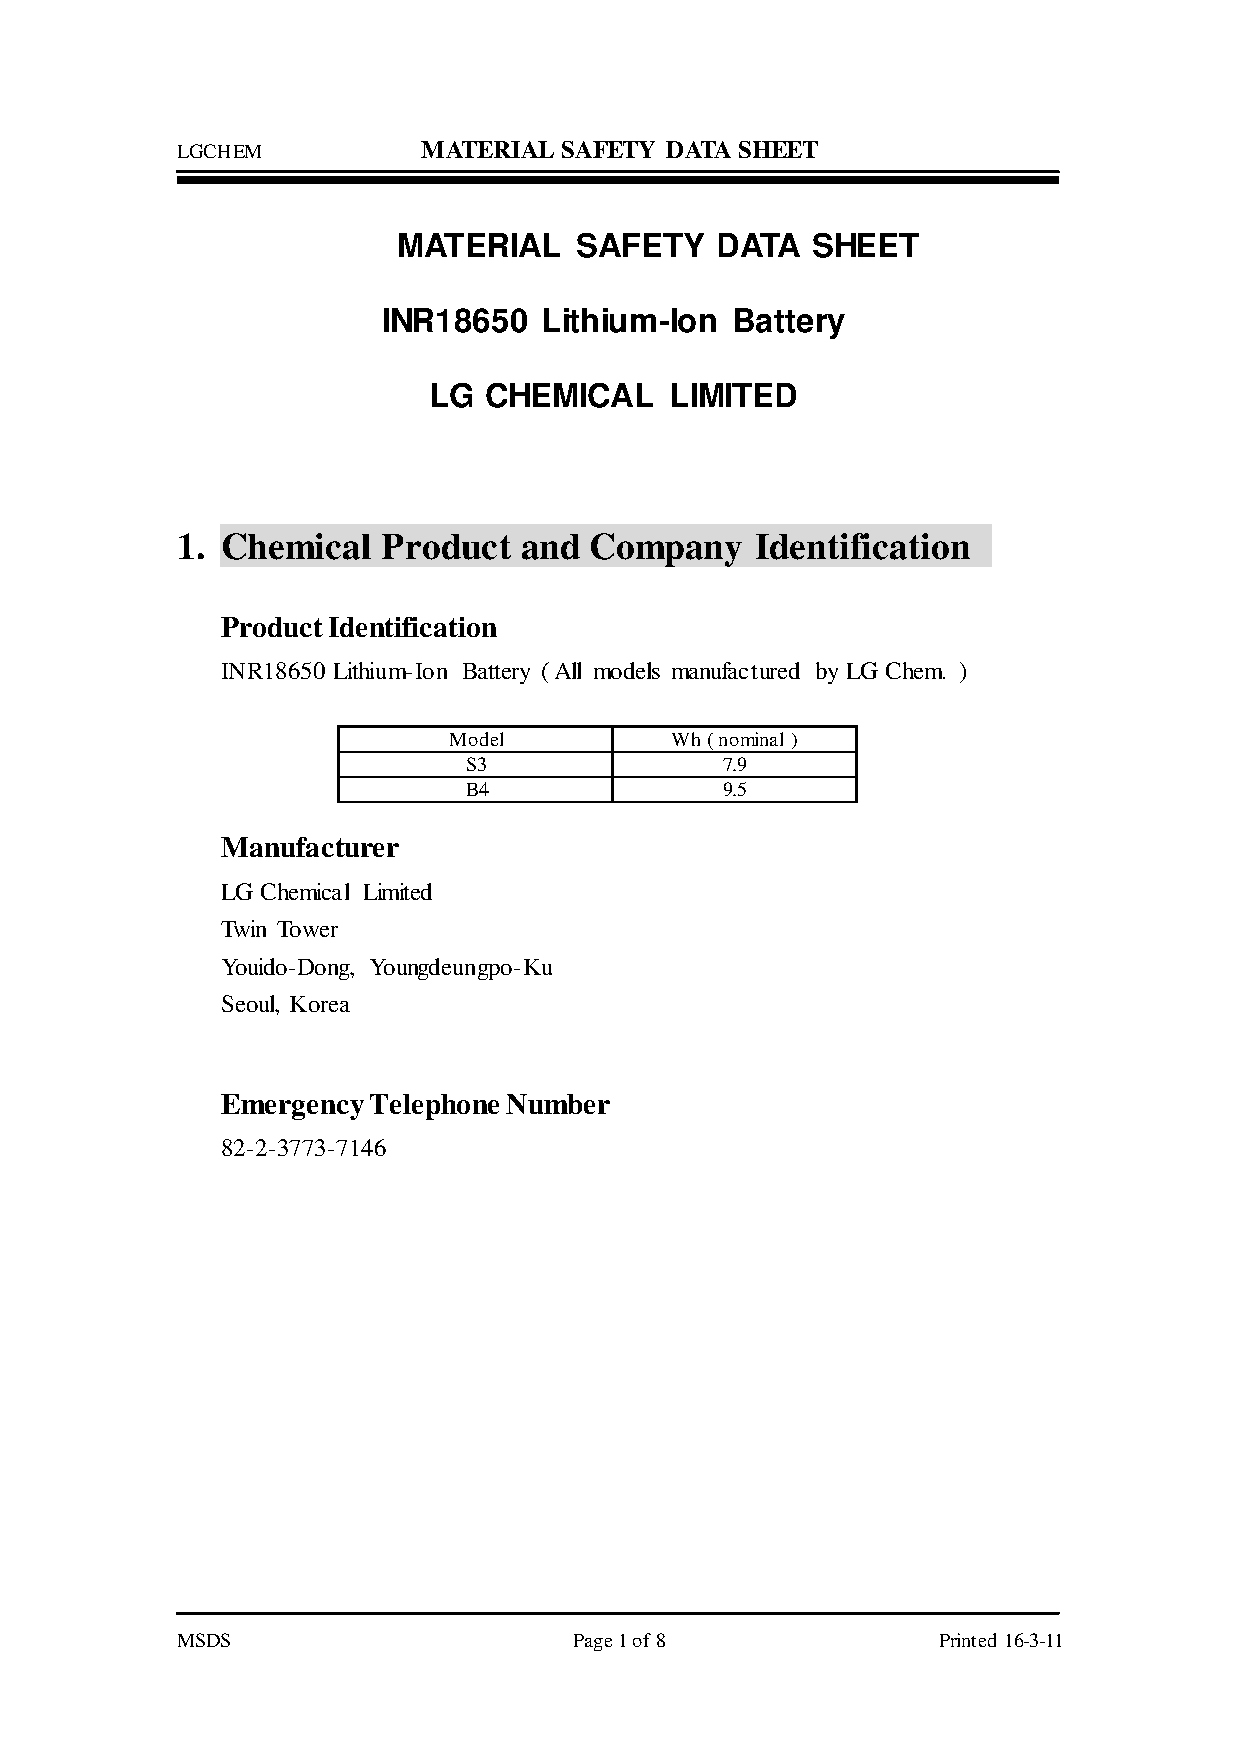
\includepdf[pages={-}]{forms/6626_1.pdf}

\subsection{5.2.D.8: Battery box information}

The 2 battery boxes are made of a fiberglass honeycomb composite. As fiberglass
is inert, it does not react with the electrolyte in a Li-ion cell or any other
potential contaminants inside the boxes. The interior of the boxes are made of
PETG, ABS and PVC plastics, all of which are inert when in contact with the
electrolyte in a Li-ion cell. Other than the electrical components
(relay, fuse, connectors, boards) the only metal used in the box is for
electrical connections, and therefore, internal shorting inside the box is
extremely unlikely.

All live connections inside the battery box are isolated at a string by string
level to ensure maximum safety. The strings are mounted via compression of the
cell holders (so as not to compress and damage the cells) on all sides so that
the strings are unable to move in any direction after the lid has been shut.
To mount the boxes to the chassis the boxes are placed into a compartment
surrounded all on sides but one by chassis members. The final side is then
enclosed via a locking hasp mechanism which is welded directly to the chassis.
Once the hasps have been locked the battery boxes have 0 degrees of freedom
and are fixed in space.

\subsection{5.2.D.9}

Not needed.

\subsection{5.2.D.10: Battery Approval Form}

See attached form.

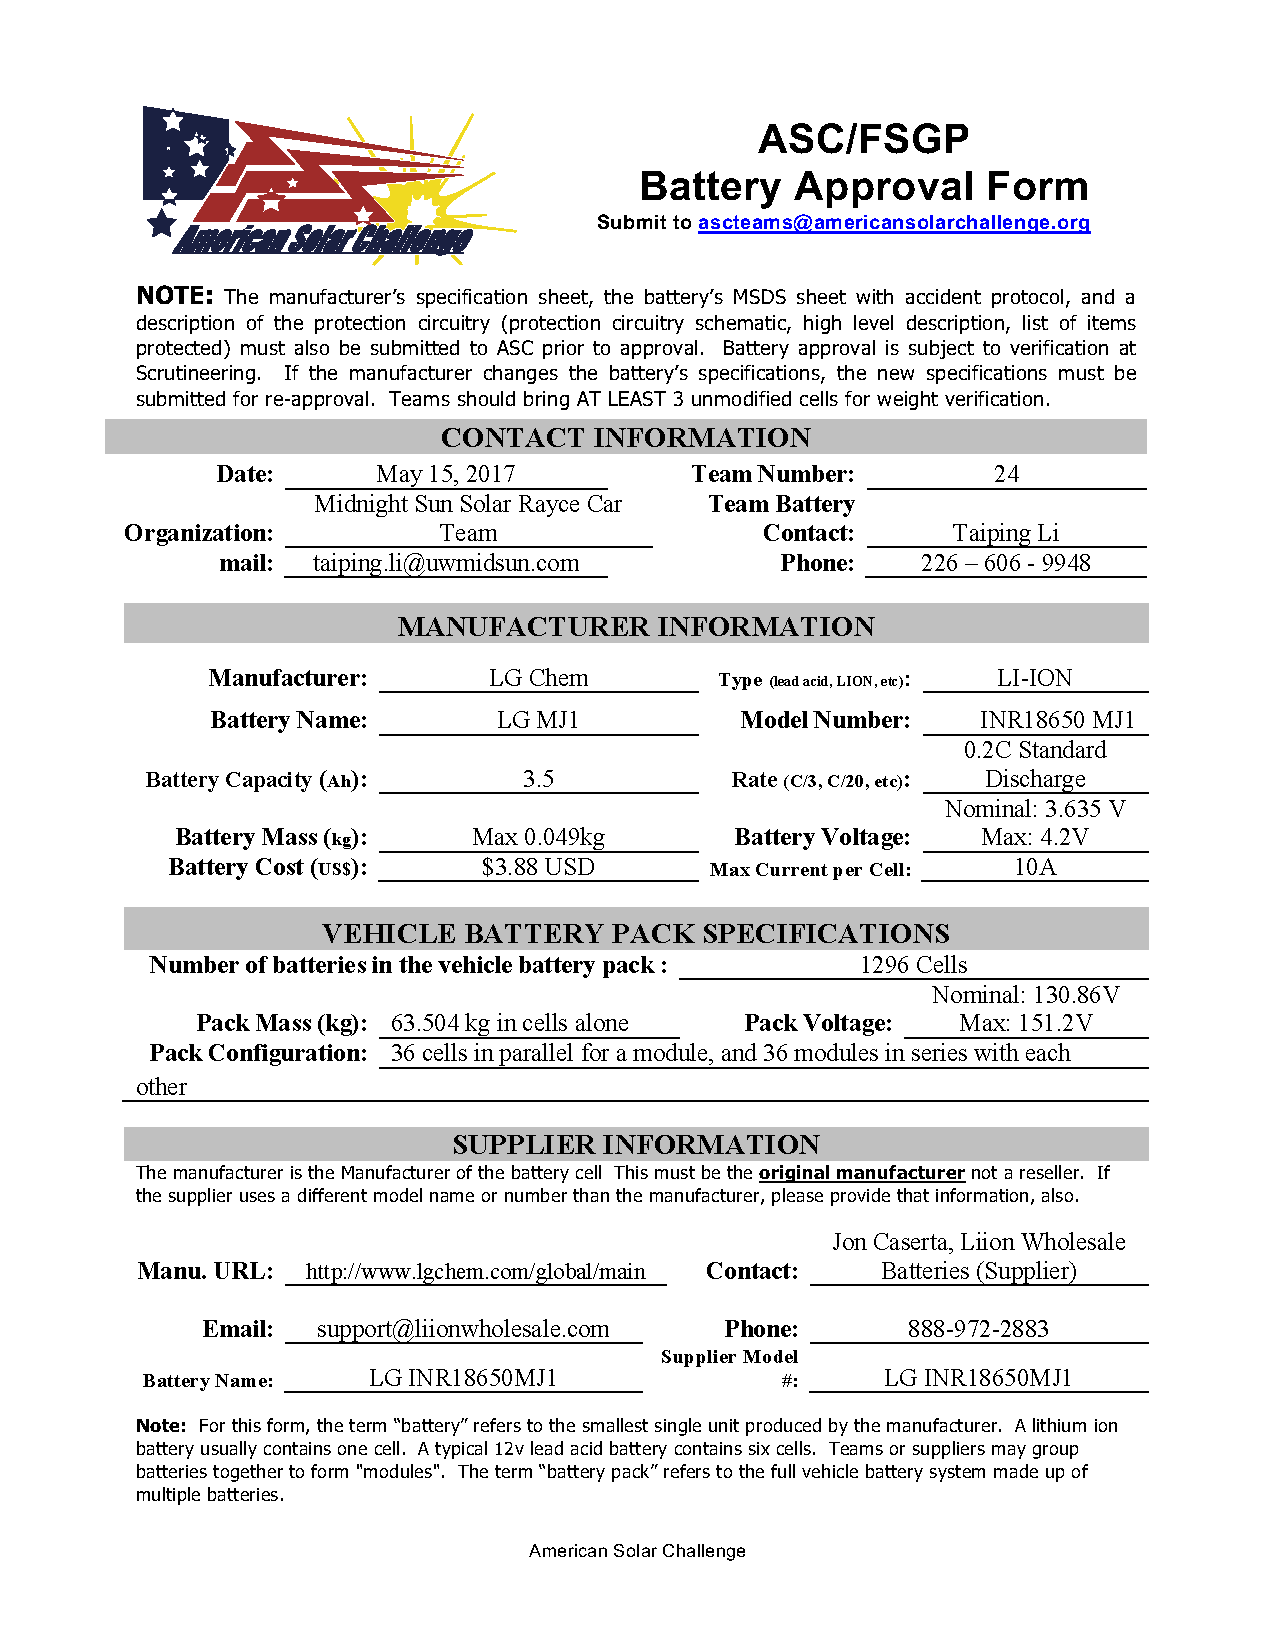
\includepdf[pages={-}]{forms/battery_approval_form.pdf}


\begin{table}[!htbp]
\centering
\begin{tabular}{|l|l|l|}
\hline
\multirow{4}{*}{5.2.D.1} & Manufacturer Name                     & LG Chemical Limited                                                                                                                   \\ \cline{2-3}
                         & Manufacturer Contact                  & \begin{tabular}[c]{@{}l@{}}Jon Caserta, Liion Wholesale Batteries (Supplier)\\ support@liionwholesale.com\\ 888-972-2883\end{tabular} \\ \cline{2-3}
                           & Cell Specification URL                & \url{http://vruzend.com/SpecificationINR18650MJ1.pdf}                                                                                       \\ \cline{2-3}
                         & Cell MSDS URL                         & \url{http://bigship.com/telechargement?doc=148635}                                                                                          \\ \hline
5.2.D.2                  & Stock Number                          & INR18650 MJ1                                                                                                                          \\ \hline
5.2.D.3                  & Cell \& Module Voltage                & \begin{tabular}[c]{@{}l@{}}3.635 V (nominal)\\ 4.200 V (max)\end{tabular}                                                               \\ \hline
5.2.D.4                  & Bus Voltage                           & \begin{tabular}[c]{@{}l@{}}130.86 V (nominal)\\ 151.2 V (max)\end{tabular}                                                              \\ \hline
\multirow{3}{*}{5.2.D.5} & Cells per module                      & 36                                                                                                                                    \\ \cline{2-3}
                         & Modules per string                    & 36                                                                                                                                    \\ \cline{2-3}
                         & Strings in parallel                   & 1                                                                                                                                     \\ \cline{2-3}
                         & Total cell count                      & 1296                                                                                                                                  \\ \hline
  \multirow{3}{*}{5.2.D.6} & Capacity (kWh)                        & $\frac{3.5 \text{ Ah} \times 130.86 \text{ V} \times 36 \text{ modules}}{1000 \text{ Wh}} = 16.48836$                                                  \\ \cline{2-3}
                         & Weight (kg)                           & \begin{tabular}[c]{@{}l@{}}0.049 kg (max)\\ 0.049 kg \times 1296 = 63.50400 kg\end{tabular}                                           \\ \cline{2-3}
                         & Cost (USD)                            & $\$ 3.88 \times 1296 = \$ 5028.48$
                         \\ \hline
5.2.D.7                  & Spill/damage protocols and procedures & See MSDS                                                                                                                              \\ \hline
5.2.D.8                  & Battery boxes and mounting            &                                                                                                                                       \\ \hline
\end{tabular}
\end{table}


% Bibliography
%\pagebreak
%\printbibliography

% Appendix
\pagebreak
\appendix

\end{document}
